\documentclass[12pt]{article}
\usepackage{fontspec}
\usepackage{graphicx}
\usepackage{geometry}
\usepackage{float}
\usepackage{hyperref}
\usepackage{tikz}
\usepackage{polyglossia}
\setmainlanguage{farsi}
\setotherlanguage{english}
\newfontfamily\englishfont{Times New Roman}
\newfontfamily\persianfont[Script=Arabic]{XB Zar.ttf}




\geometry{a4paper, margin=2.5cm}
\usepackage{setspace}
\onehalfspacing
\usepackage{titling}
\usepackage{etoolbox}
\usepackage[backend=biber,style=numeric,sorting=none]{biblatex}
%%%%%%%%%%%%%%%%%%%%%%%%%%%%%%%%%%%%%%%%%%%%%%%%%%%%%%%%%%%%%%%%%%%%%%%%%%%%%
\makeatletter
\newcommand{\persiandigit}[1]{%
	\ifcase#1 ۰\or ۱\or ۲\or ۳\or ۴\or ۵\or ۶\or ۷\or ۸\or ۹\fi
}
\DeclareFieldFormat{labelnumber}{\persiandigit{#1}}
\makeatother
%%%%%%%%%%%%%%%%%%%%%%%%%%%%%%%%%
\newcommand{\persianordinal}[1]{%
	\ifcase#1
	\or اول%
	\or دوم%
	\or سوم%
	\or چهارم%
	\or پنجم%
	\or ششم%
	\or هفتم%
	\or هشتم%
	\or نهم%
	\or دهم%
	\or یازدهم%
	\or دوازدهم%
	\or سیزدهم%
	\or چهاردهم%
	\or پانزدهم%
	\or شانزدهم%
	\or هفدهم%
	\or هجدهم%
	\or نوزدهم%
	\or بیستم%
	\else #1\fi
}

\newcommand{\persianordinalpage}{\persianfont\persianordinal{\value{page}}}


%%%%%%%%%%%%%%%%%%%%%%%%%%%%%%%%%%%%%%%%%%%%%%%%%%%%%%%%%%%%%%%%%%%%%%%%%%%%%
\begin{filecontents}{\jobname.bib}


\end{filecontents}

\addbibresource{\jobname.bib}

\defbibheading{bibliography}[]{%
	\begin{RTL}
		\section*{مراجع}
	\end{RTL}
}

%%%%%%%%%%%%%%%%%%%%%%%%%%%%%%%%%%%%%%%%%%%%%%%%%%%%%%%%%%%%%%%%%%%%%%%%%%%%%

\begin{document}
	
	% ==============================
	% Title Page
	% ==============================
	\begin{titlepage}
		\centering
		\vspace*{1cm}
		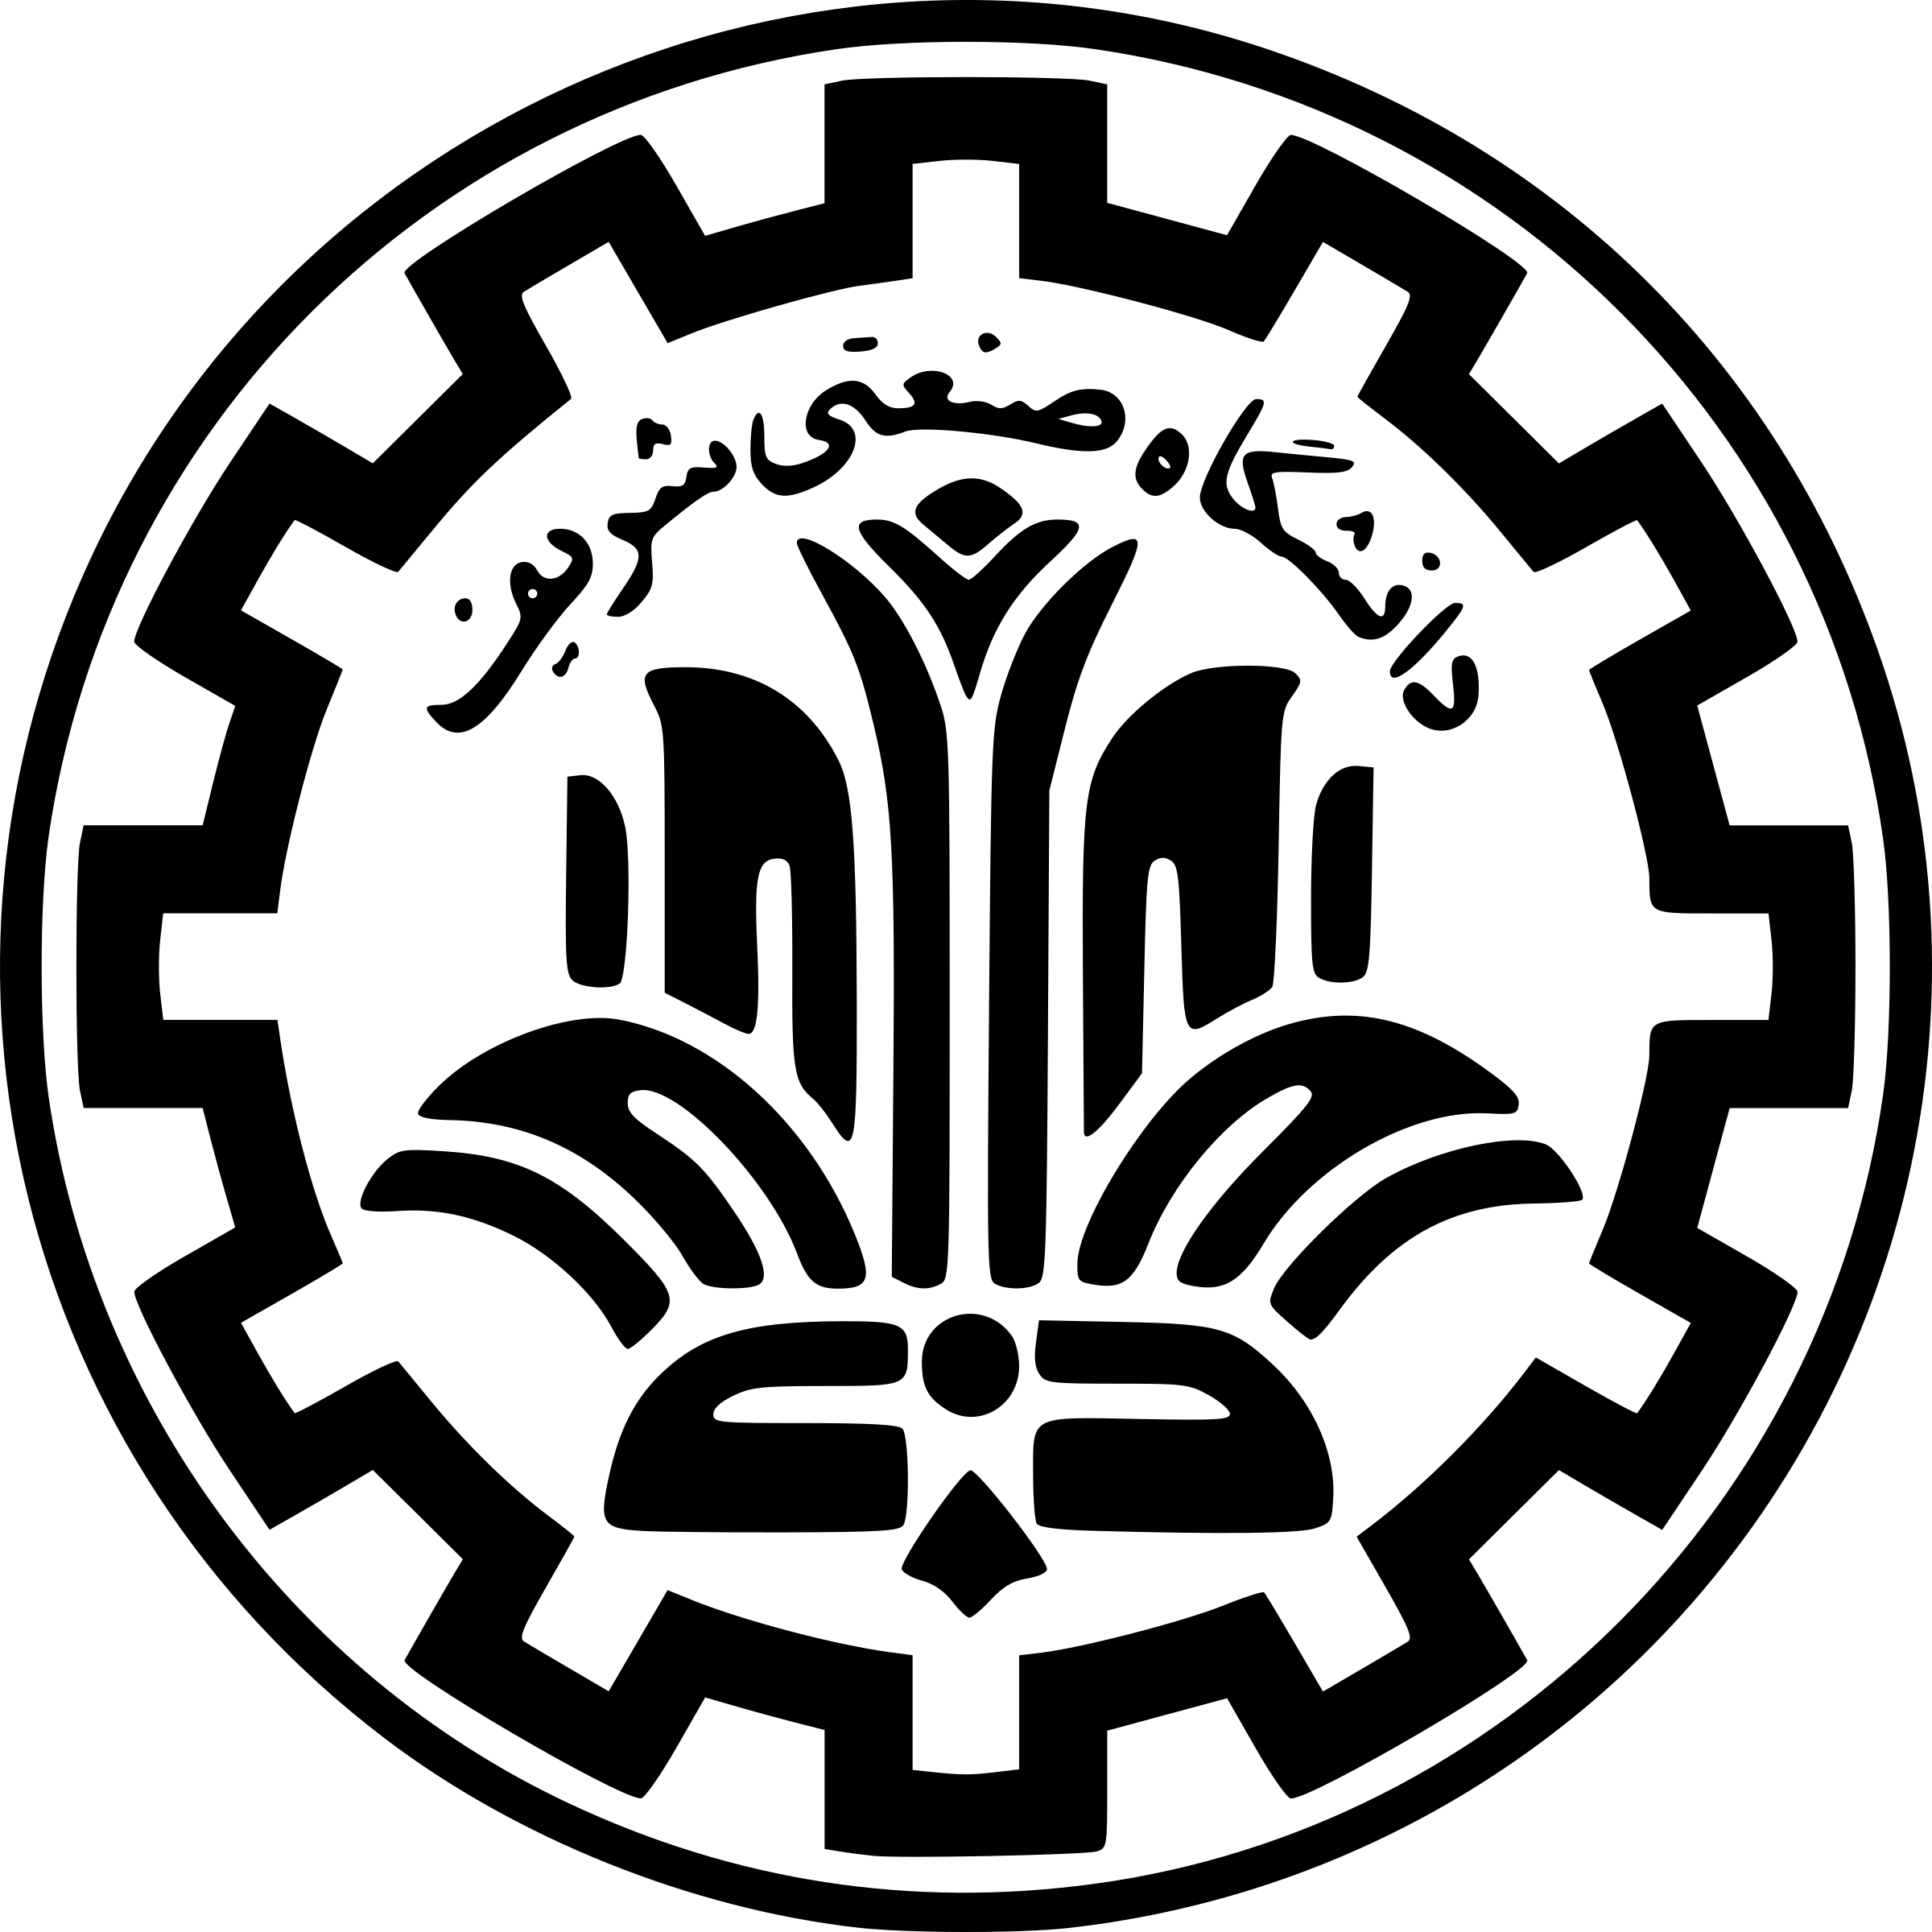
\includegraphics[width=4cm]{sharif.png}\\[1.5cm]
		{\Large\textbf{دانشگاه صنعتی شریف}}\\[0.5cm]
		{\large\textbf{دانشکده‌ی مهندسی کامپیوتر}}\\[1.5cm]
		{\Huge\textbf{گزارش کار آزمایشگاه}}\\[0.5cm]
		{\LARGE\textbf{آزمایشگاه سیستم‌های عامل}}\\[2cm]
		
		\textbf{گزارش آزمایش شماره ۶}\\
		(مدیریت حافظه)
		
		\vfill
		\begin{tabular}{rl}
			\textbf{شماره‌ی گروه:} & ۲۰ \\
			\textbf{گروه:} &
			ارشیا یوسف‌نیا (۴۰۱۱۱۰۴۱۵) \\
			& محمدعارف زارع زاده (۴۰۱۱۰۶۰۱۷) \\
			\textbf{استاد درس:} & دکتر بیگی \\
			\textbf{تاریخ:} & تابستان ۱۴۰۴ \\
		\end{tabular}
	\end{titlepage}
	
	% ==============================
	% Persian Ordinal Page Numbering
	% ==============================
	\clearpage
	\setcounter{page}{1}
	\renewcommand{\thepage}{\persianordinalpage}
	
	\tableofcontents
	\clearpage
	\listoffigures
	% \clearpage
	% \listoftables
	
	% ==============================
	% Switch to Persian Digits (۱, ۲, ۳, ...)
	% ==============================
	\clearpage
	\setcounter{page}{1}
	\pagenumbering{arabic}
	\renewcommand{\thepage}{\persianfont\arabic{page}}
	
	
	% ==============================
	% Main Content
	% ==============================
        \section{شرح آزمایش}
        \subsection{استفاده از فراخوانی‌های \textenglish{malloc} و \textenglish{free}}
        

        خروجی دستور
        \textenglish{malloc}
        یک پوینتر از نوع
        \textenglish{void *}
        است. این پوزنتر، به آدرسی که دستور
        \textenglish{malloc}
        به اندازه‌ی خواسته شده حافظه را آماده کرده اشاره می‌کند.
        با تغییر نوع پویتر (یا همان
        \textenglish{casting})
        می‌توان نوع این پونتر را به پوینتر مناسب تغییر داد و به این صورت 
        فیلدهای یک 
        \textenglish{struct}
        را تغییر داد یا درصورت نیاز کارهای دیگری کرد.

        کد خواسته شده را در شکل 
        \ref{im1}
        می‌توانید مشاهده کنید. در این کد، ابتدا با دستور
        \textenglish{malloc}
        به اندازه‌ی کافی حافظه را برای یک 
        \textenglish{instance}
        از آن
        \textenglish{struct}
        آماده کرده و سپس به فیلدهای آن مقدار دلخواهی می‌دهیم. سپس با دستور
        \textenglish{free}
        سعی می‌کنیم آن بخش از حافظه را آزاد کرده، و سپس سعی می‌کنیم مثل قبل، فیلدهای آن را پرینت کنیم. در دفعه‌ی دوم، یا باید به ارور خورده، یا باید مقدار فیلدها تغییر کند و مقادیری تصادفی داشته باشد.

        \begin{figure}[H]
		\centering
		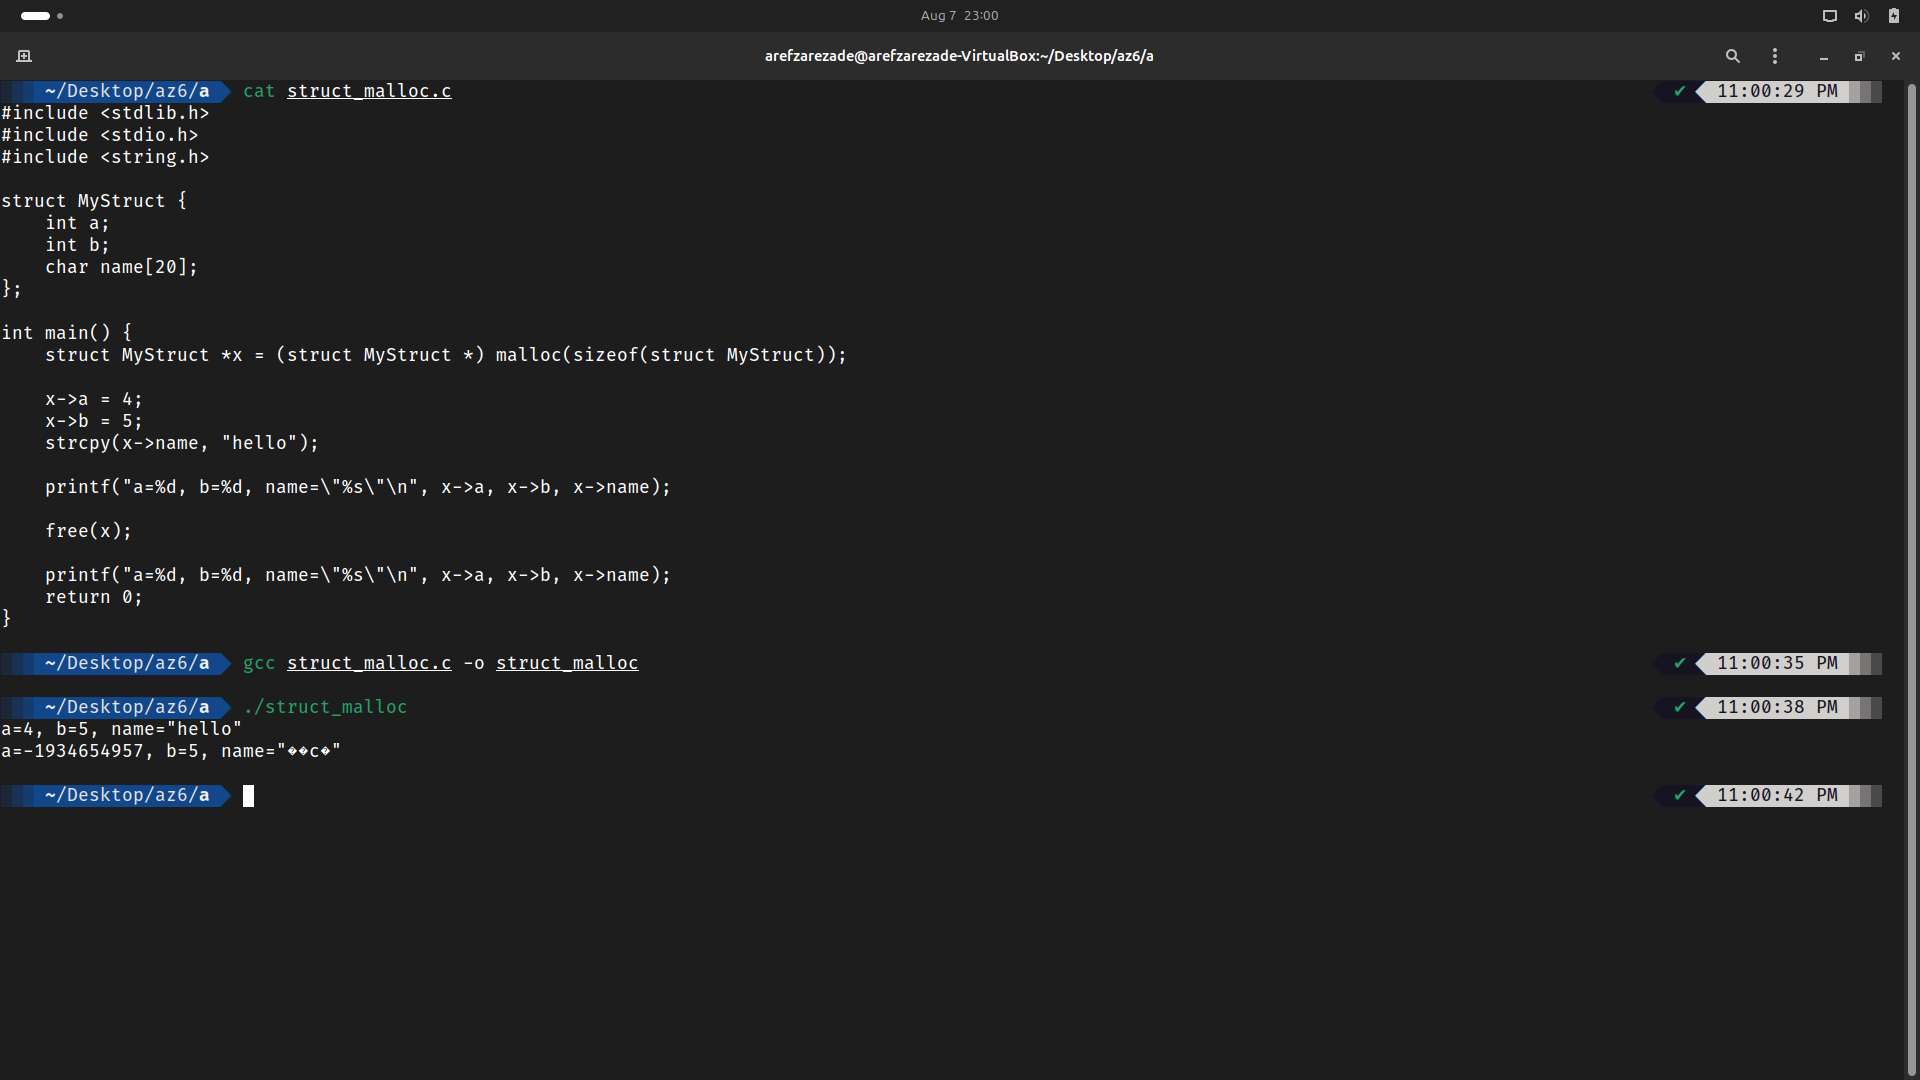
\includegraphics[width=0.8\textwidth]{report6-resources/1.png}
		\caption{کد کار کردن با دستورات \textenglish{malloc} و \textenglish{free}}
            \label{im1}
	\end{figure}

        \subsection{مشاهده ی وضعیت حافظه ی پردازه ها}

        ابتدا با کمک دستور
        \textenglish{man ps}،
        هر یک از ستون‌ها را پیدا کرده، و سپس معنای هرکدام را می‌نویسیم. در کنار هرکدام، یک تصویر از صفحه‌ی 
        \textenglish{man}
        مربوط به آن ستون را نشان می‌دهیم.

        \begin{itemize}
        \item ستون \textenglish{user}:
        این ستون مطابق شکل 
        \ref{im2}
        نام کاربری که پردازه از طرف او اجرا می‌شود را می‌نویسد. 
        همانطور که از شکل
        \ref{im7}
        می‌توان مشاهده کرد، اگر پردازه از طرف سیستم اجرا می‌شود، مقدار آن
        \textenglish{root}
        می‌باشد.

        \begin{figure}[H]
		\centering
		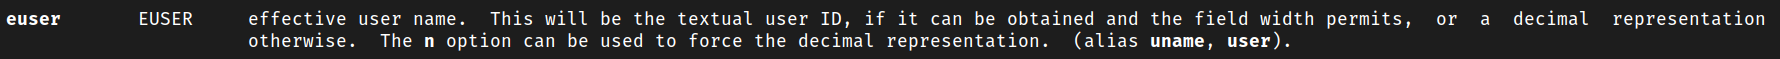
\includegraphics[width=0.8\textwidth]{report6-resources/2.png}
		\caption{ستون \textenglish{user} در دستور داده شده طبق صفحه‌ی \textenglish{man ps}}
            \label{im2}
	\end{figure}

        \item ستون \textenglish{vsz}:
        این ستون مطابق شکل 
        \ref{im3}
        میزان حافظه‌ی مجازی مربوط به آن پردازه را برحسب کیلوبایت بیان می‌کند.

        \begin{figure}[H]
		\centering
		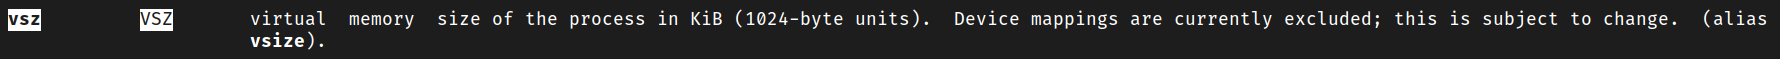
\includegraphics[width=0.8\textwidth]{report6-resources/3.png}
		\caption{ستون \textenglish{vsz} در دستور داده شده طبق صفحه‌ی \textenglish{man ps}}
            \label{im3}
	\end{figure}

        \item ستون \textenglish{rss}:
        این ستون مطابق شکل 
        \ref{im4}
        میزان حافظه‌ی فیزیکی که پردازه در حال حاضر استفاده می‌کند را نشان می‌دهد. واضح است که مقدار این ستون همواره کمتر یا مساوری ستون
        \textenglish{vsz}
        باید باشد. این موضوع در شکل
        \ref{im7}
        قابل مشاهده است.

        \begin{figure}[H]
		\centering
		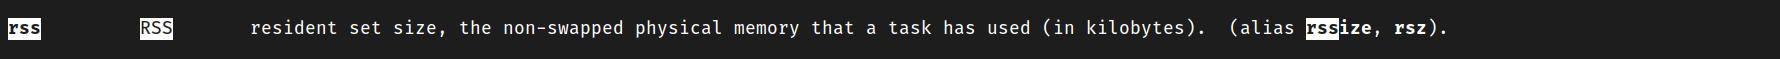
\includegraphics[width=0.8\textwidth]{report6-resources/4.png}
		\caption{ستون \textenglish{rss} در دستور داده شده طبق صفحه‌ی \textenglish{man ps}}
            \label{im4}
	\end{figure}

        \item ستون \textenglish{pmem}:
        این ستون مطابق شکل 
        \ref{im5}
        درصدی از کل حافظه را که پردازه در حال حاضر دارد استفاده می‌کند را نشان می‌دهد. بدیهی است که مقدار آن باید متناسب با 
        \textenglish{rss}
        باشد، و این موضوع در شکل
        \ref{im7}
        قابل مشاهده است.

        \begin{figure}[H]
		\centering
		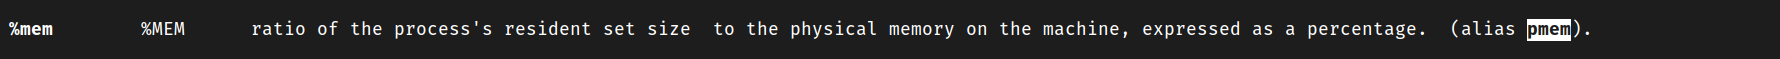
\includegraphics[width=0.8\textwidth]{report6-resources/5.png}
		\caption{ستون \textenglish{pmem} در دستور داده شده طبق صفحه‌ی \textenglish{man ps}}
            \label{im5}
	\end{figure}

        \item ستون \textenglish{fname}:
        این ستون مطابق شکل 
        \ref{im6}
        \textenglish{8}
        بایت (که در اکثر اوثات 
        \textenglish{8}
        حرف است) اول نام فایل
        \textenglish{executable}
        مربوط به آن پردازه را می‌نویسد. به بیان دیگر، برنامه‌ای که اجرای آن باعث ایجاد این پردازه شده است را نشان می‌دهد.


        \begin{figure}[H]
		\centering
		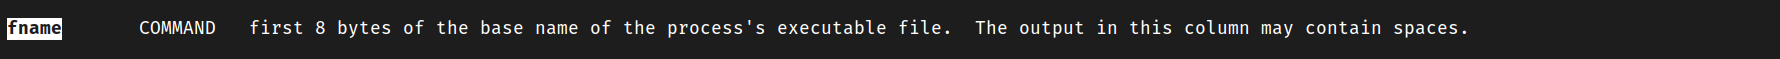
\includegraphics[width=0.8\textwidth]{report6-resources/6.png}
		\caption{ستون \textenglish{fname} در دستور داده شده طبق صفحه‌ی \textenglish{man ps}}
            \label{im6}
	\end{figure}

        \end{itemize}

        همچنین در شکل
        \ref{im7}
        می‌توانید یک نمونه از اجرای دستور داده شده را مشاهده کنید.

        \begin{figure}[H]
		\centering
		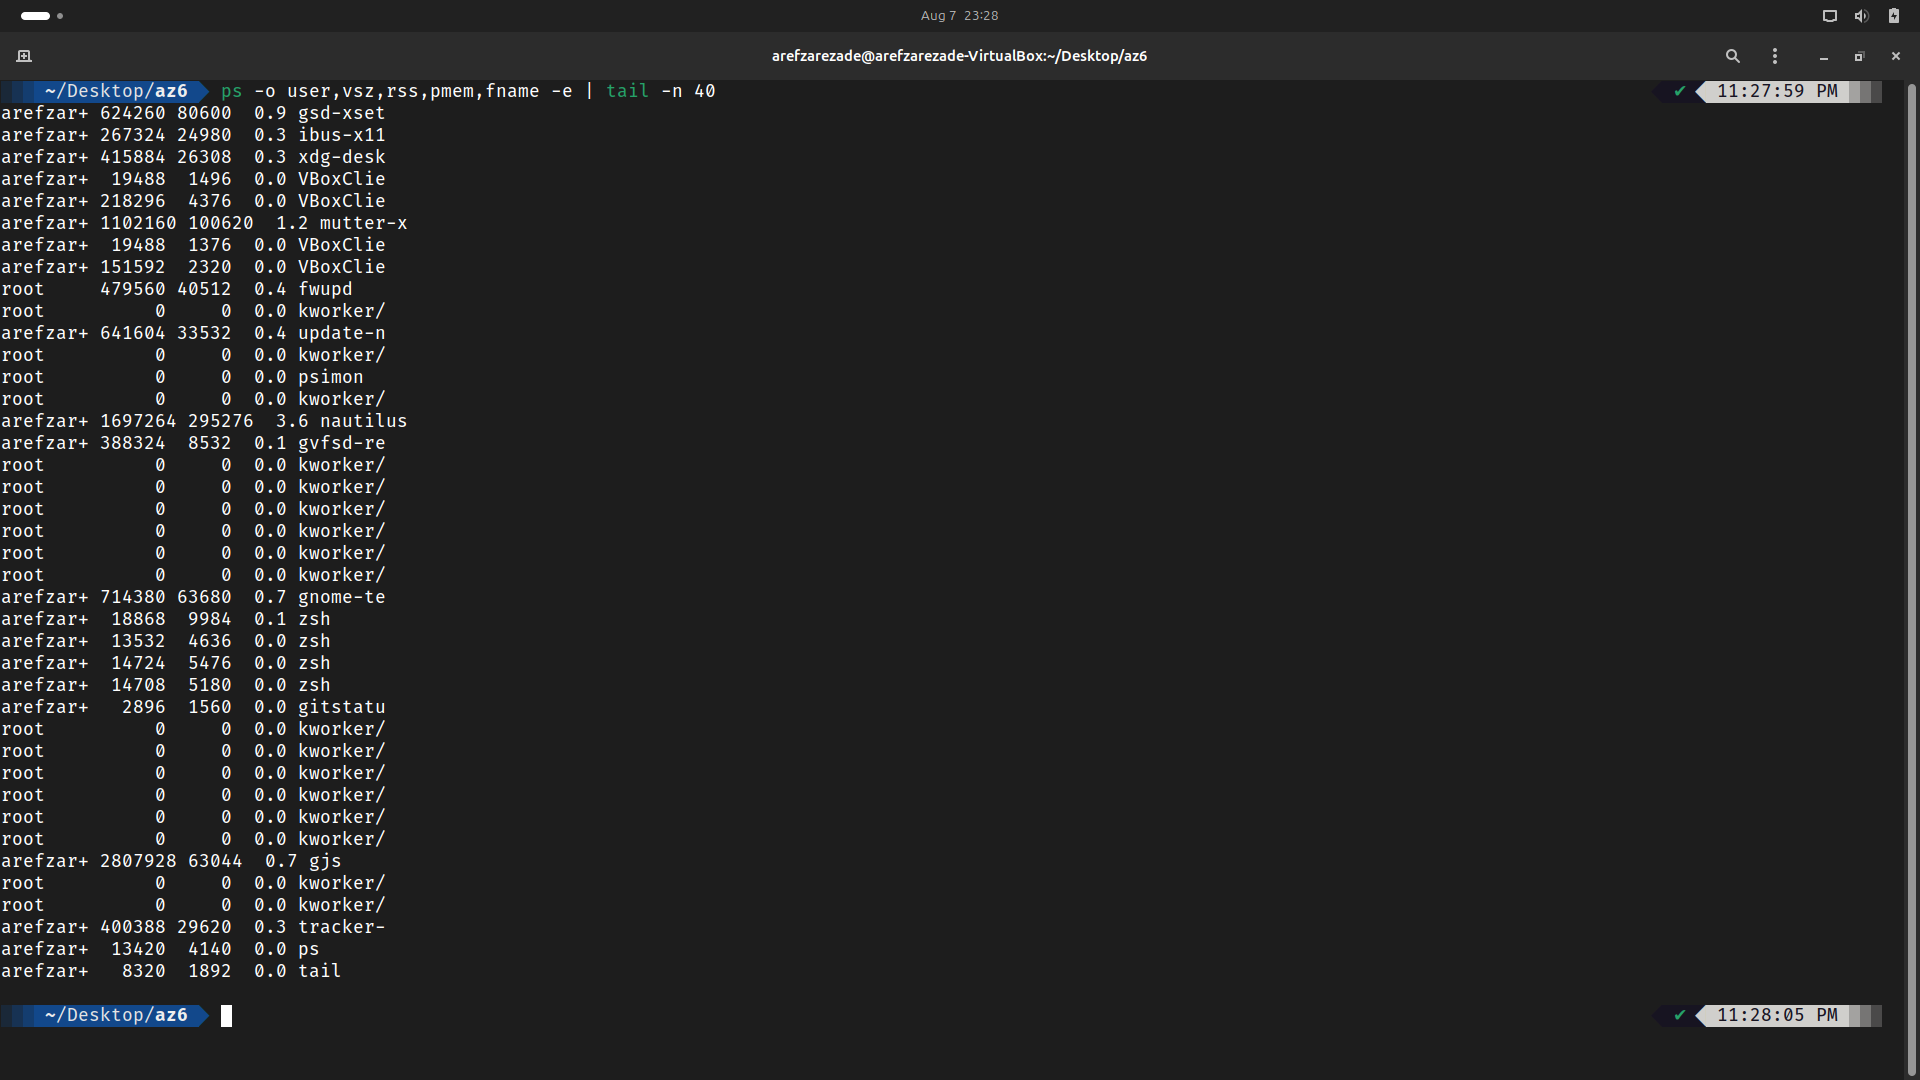
\includegraphics[width=0.8\textwidth]{report6-resources/7.png}
		\caption{اجرای دستور \textenglish{ps} با ستون‌های خواسته شده}
            \label{im7}
	\end{figure}


        \subsection{اجزای حافظه‌ی یک پردازه}

        در شکل 
        \ref{im8}
        می‌توان محل قرارگیری دستور
        \textenglish{ls}
        درون فایل سیستم و همچنین میزان تخصیص حافظه به بخش‌های گفته شده را مشاهده کرد.

        \begin{figure}[H]
		\centering
		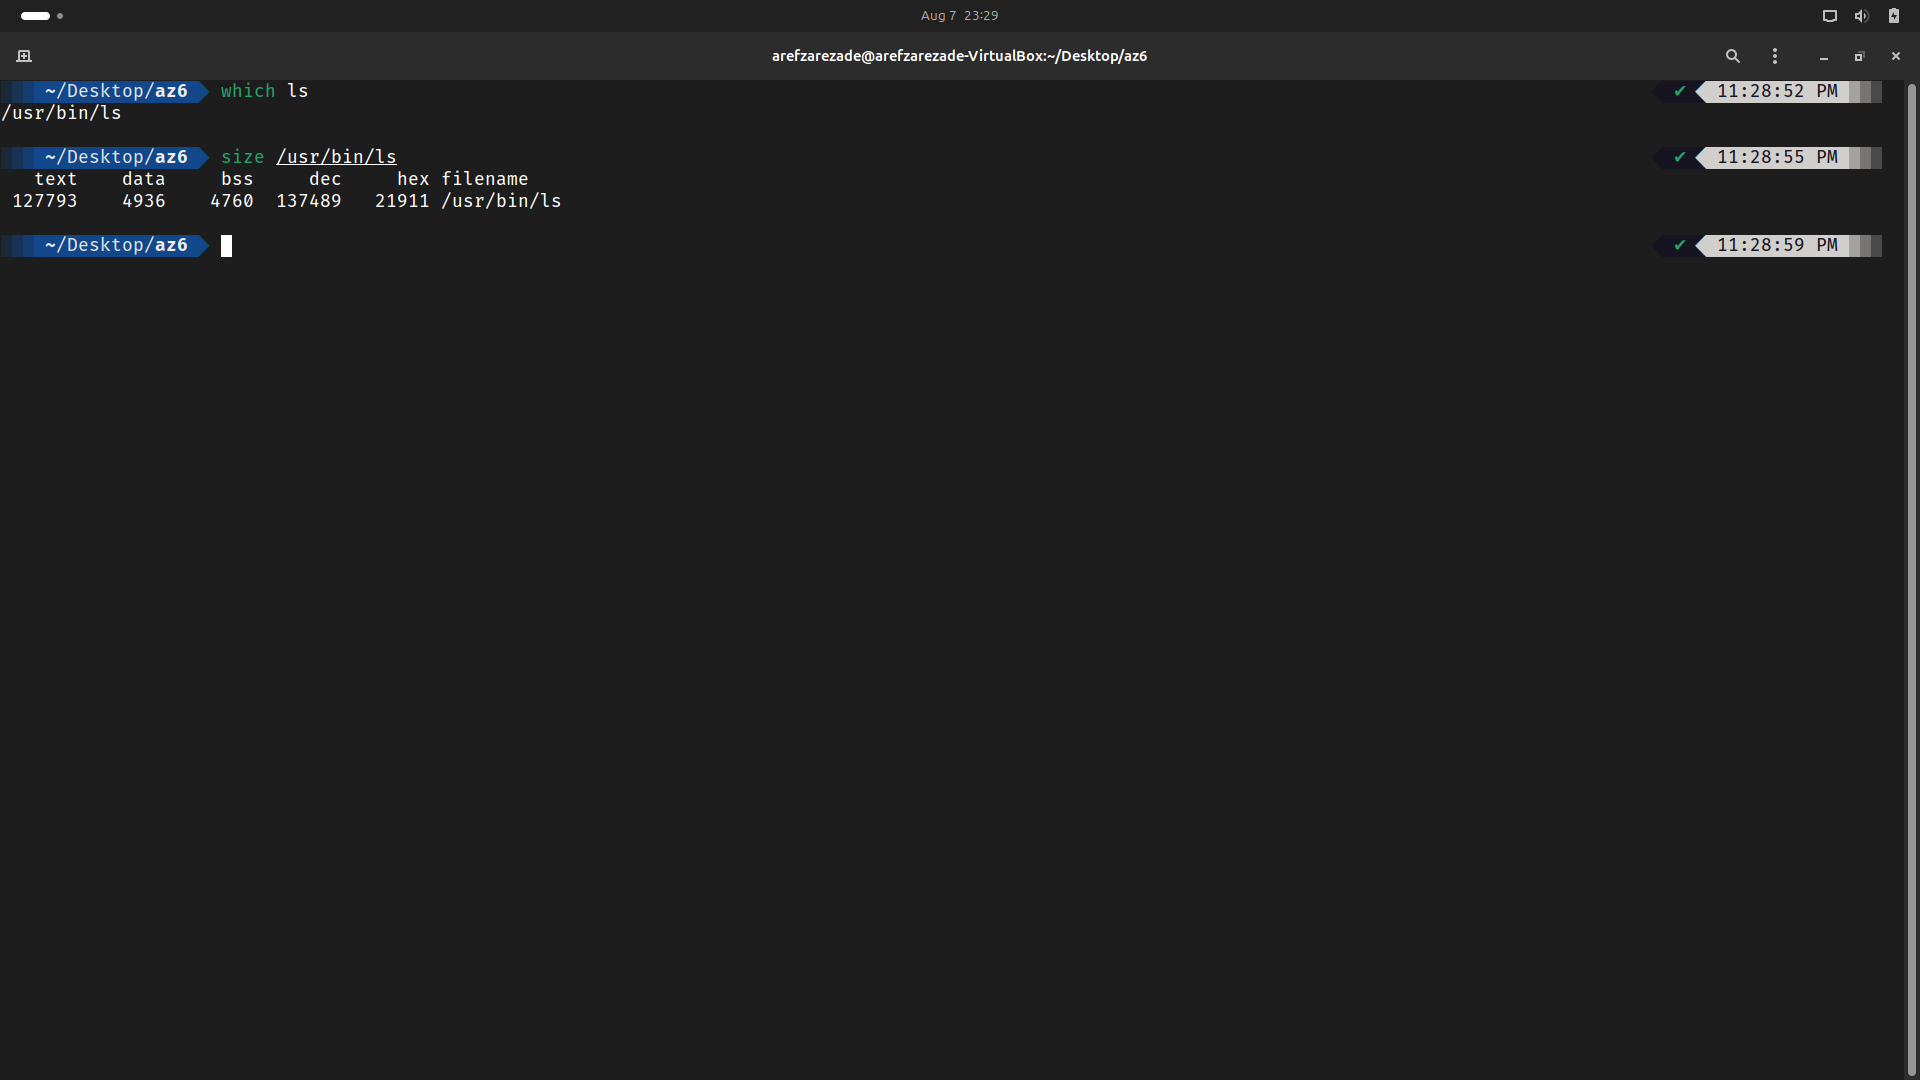
\includegraphics[width=0.8\textwidth]{report6-resources/8.png}
		\caption{محل قرارگیری دستور \textenglish{ls} و حافظه‌ی اختصاص داده شده به اجزای آن}
            \label{im8}
	\end{figure}

        همانطور که می‌توان مشاهده کرد، مقادیر
        \textenglish{data}
        و 
        \textenglish{text}
        و
        \textenglish{bss}
        را می‌توان مشاهده کرد. همچنین حافظه‌ی مربوط به 
        \textenglish{initialized data}
        با اینکه به طور مستقیم داده نشده است، با کمک اجزای دیگر می‌توان آن را به دست آورد (اختلاف
        \textenglish{data}
        و 
        \textenglish{bss}).

        اما مقادیر
        \textenglish{command-line arguements and environment variables}
        (به خاطر متفاوت بودن در هربار اجرای دستور)
        و همچنین 
        \textenglish{stack}
        و
        \textenglish{heap}
        (به خاطر متغیر بودن و همواره کم یا زیاد شدنشان حین اجرای دستور)
        هنگام اجرای دستور
        \textenglish{size}
        گزارش نمی‌شوند.

        \subsection{اشتراک حافظه}

        در شکل 
        \ref{im9}
        می‌توان کتابخانه‌های مشترک مورد استفاده‌ی دستور
        \textenglish{ls}
        را مشاهده کرد. همچنین در شکل
        \ref{im10}
        کتابخانه‌های مشترک تعدادی دستور دیگر (\textenglish{nano} و \textenglish{touch} و \textenglish{size}) را مشاهده کرد.

        \begin{figure}[H]
		\centering
		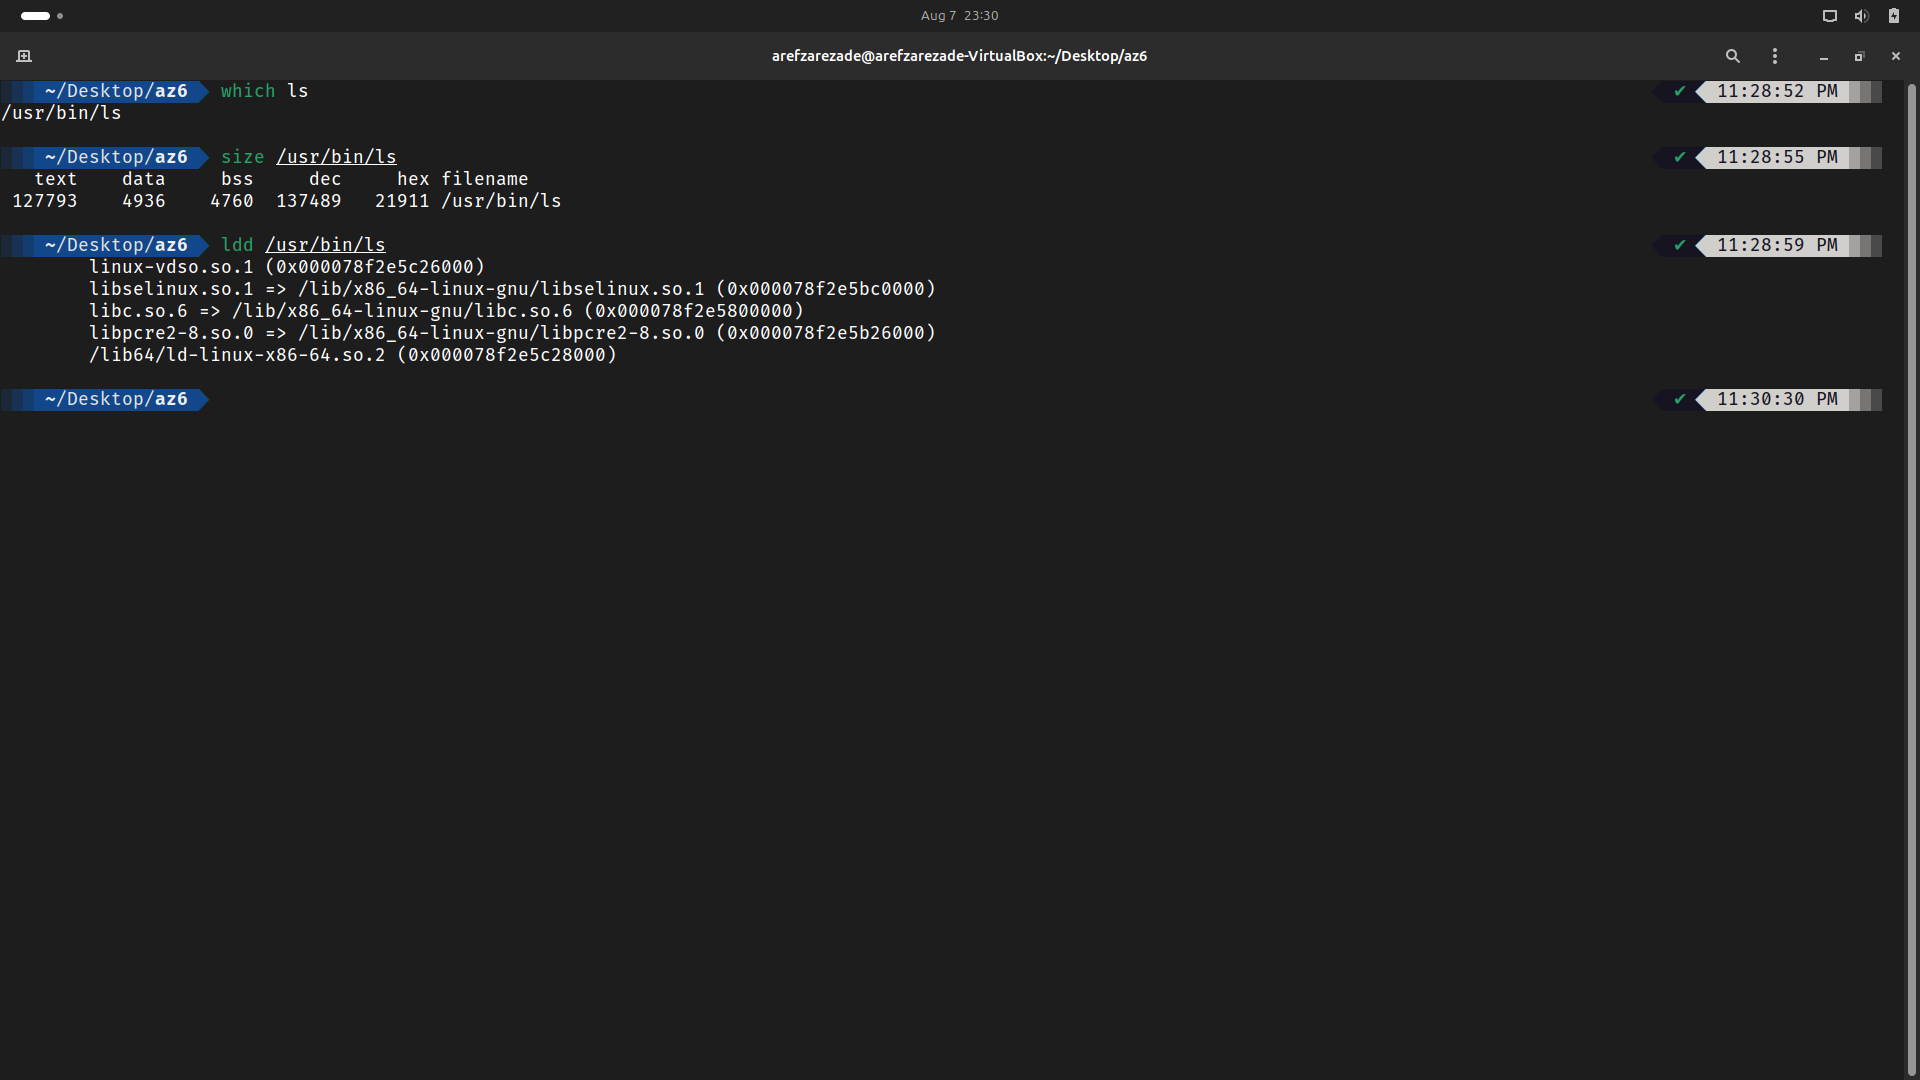
\includegraphics[width=0.8\textwidth]{report6-resources/9.png}
		\caption{کتابخانه‌های مشترک مورد استفاده توسط دستور \textenglish{ls}}
            \label{im9}
	\end{figure}

        \begin{figure}[H]
		\centering
		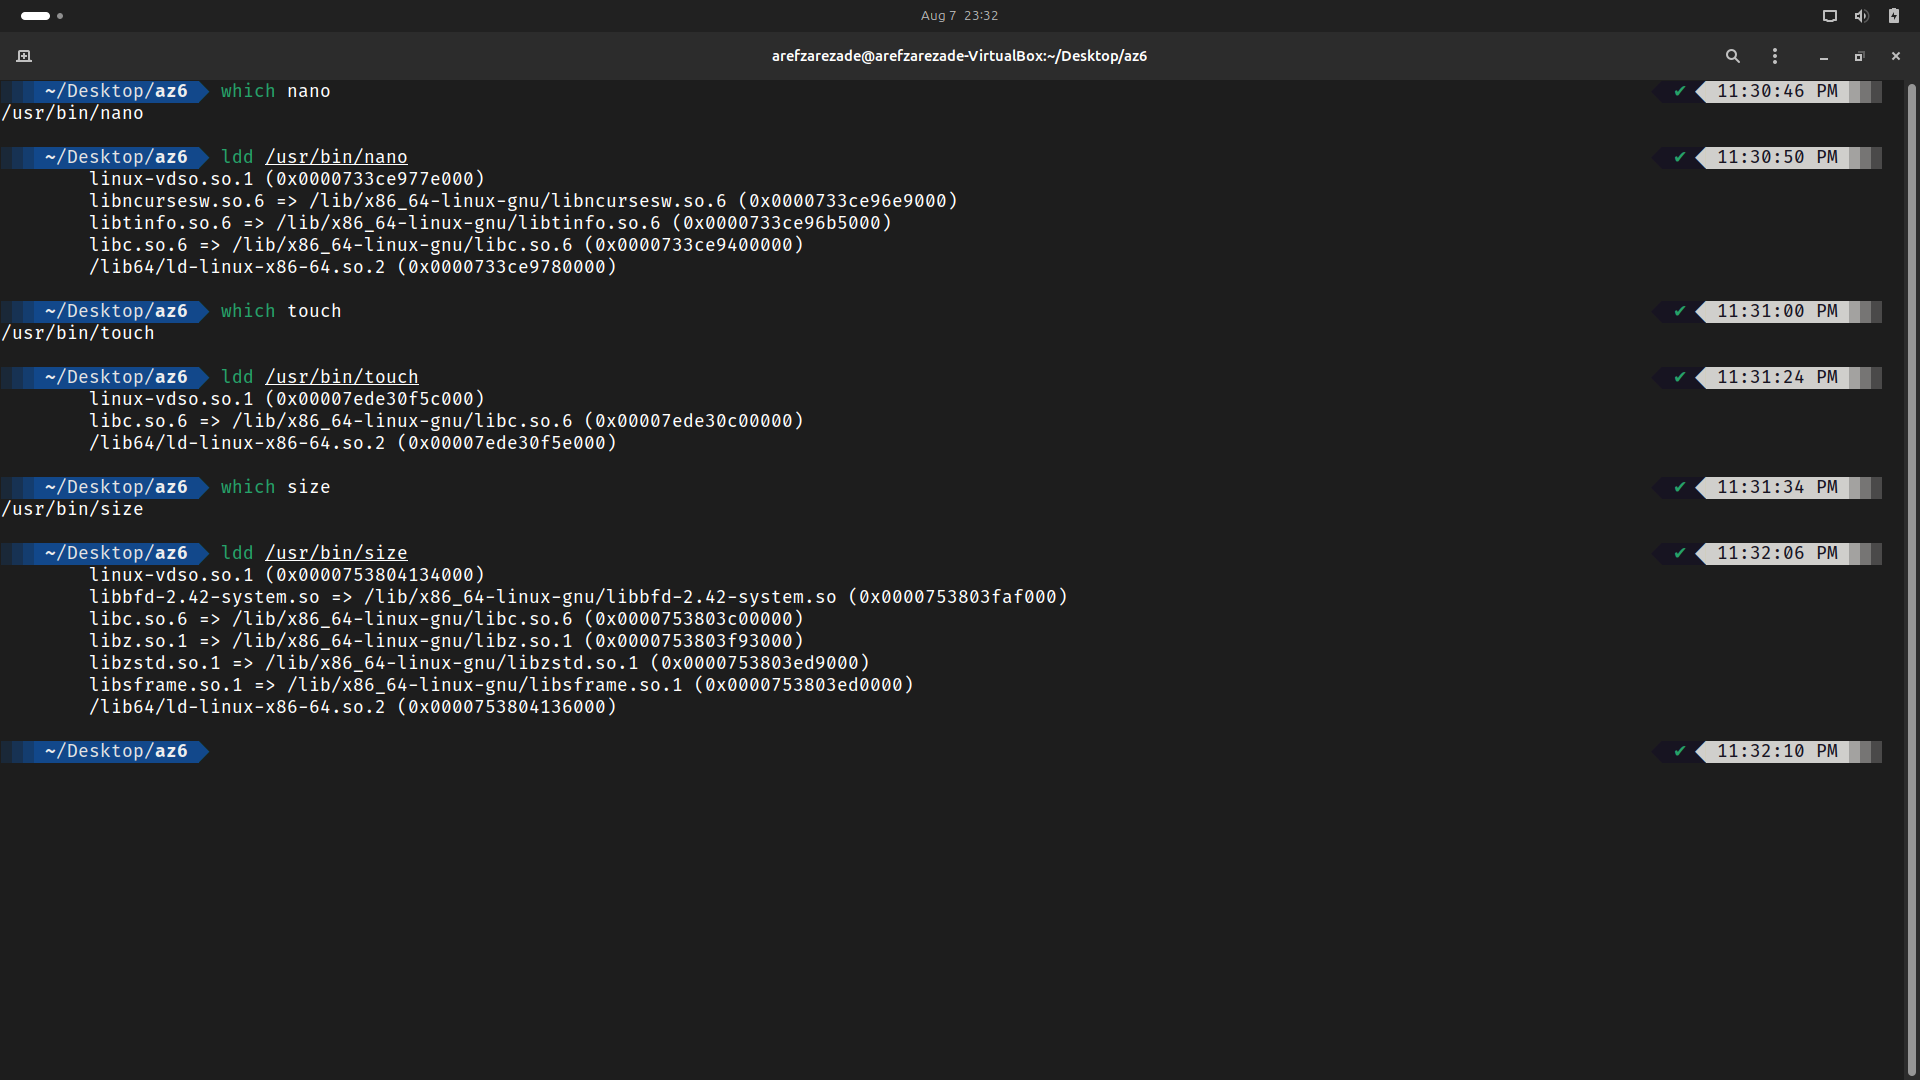
\includegraphics[width=0.8\textwidth]{report6-resources/10.png}
		\caption{کتابخانه‌های مشترک مورد استفاده توسط تعدادی دستور دیگر}
            \label{im10}
	\end{figure}

        همانطور که می‌توان مشاهده کرد، بین اینها، بعضی کتابخانه‌ها مانند
        \textenglish{linux-vsdo.so.1}
        در همه‌ی دستورات تست شده مورد استفاده قرار گرفته اند، و سیستم عامل به جای اینکه هربار جداگانه آنها را وارد حافظه کند، بهتر است یک بار وارد حافظه کرده و بین آنها بخش
        \textenglish{text}
        را به اشتراک بگذارد.

        \subsection{آدرس‌های بخش‌های مختلف پردازه}

        

        نکته: خواسته‌های این بخش در 
        \textenglish{pdf}
        داده شده و همچنین گیتهاب، تفاوت‌های جزئی دارد. طبق آخرین پیام کوئرا در زمان نوشتن گزارش، طبق صورت آزمایش موجود در گیتهاب به خواسته‌ها جواب می‌دهیم.

        \begin{itemize}
        \item 
        کد گفته شده و همچنین اجرای آن را در شکل 
        \ref{im11}
        می‌توانید مشاهده کنید. همانطور که در این شکل می‌توان دید، مقدار 
        \textenglish{etext}
        که انتهای بخش
        \textenglish{text}
        است از همه کوچکتر است. سپس مقدار
        \textenglish{edata}
        که آدرس انتهای بخش 
        \textenglish{data}
        که همان انتهای
        \textenglish{initialized data}
        است کوچکتر است، و درنهایت مقدار
        \textenglish{end}
        که همان آدرس انتهای بخش
        \textenglish{uninitialized data}
        است از همه بزرگتر است. این موضوع با موارد گفته شده در صورت آزمایش در تطابق است.

        \begin{figure}[H]
		\centering
		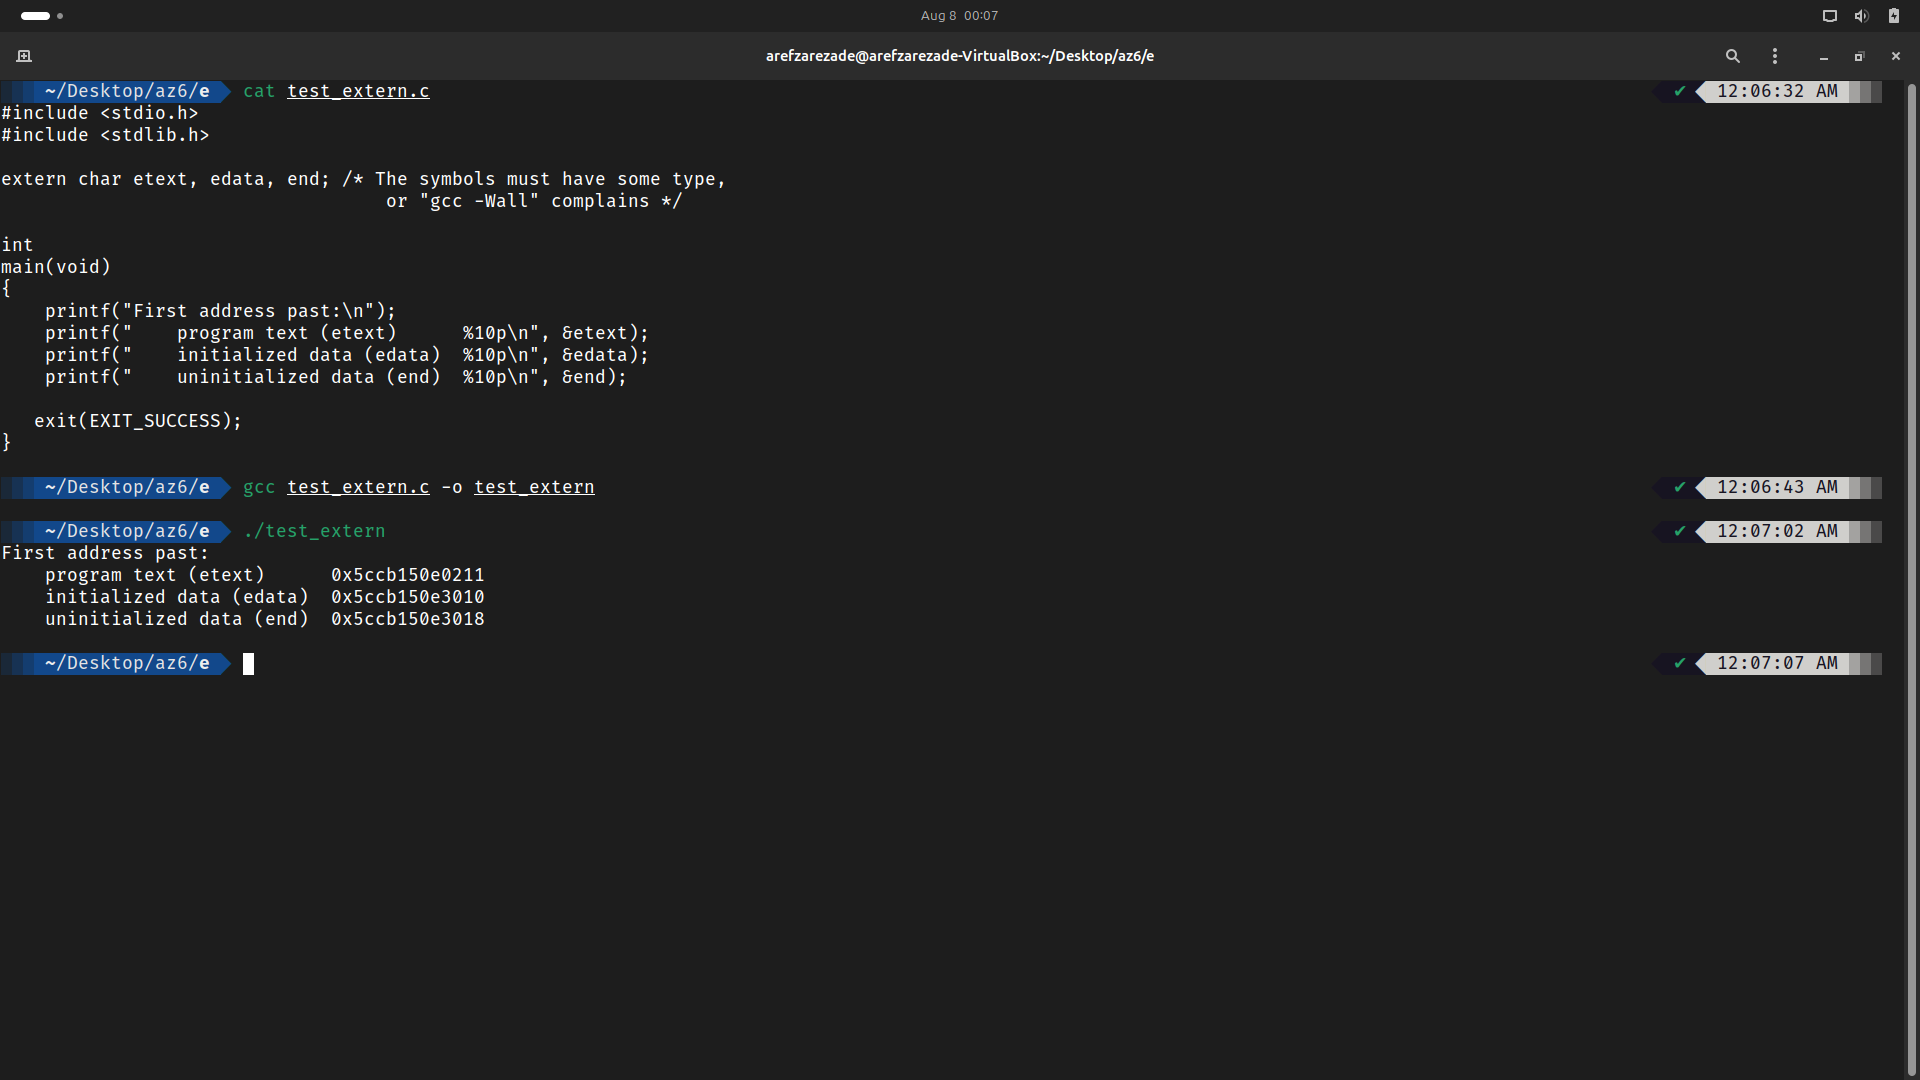
\includegraphics[width=0.8\textwidth]{report6-resources/11.png}
		\caption{کد انتهای صفحه‌ی \textenglish{man etext}}
            \label{im11}
	\end{figure}

        دلیل اینکه در کامنت به اینها 
        \textenglish{symbol}
        گفته شده است، این است که اینها متغیر معمولی نیستند، بلکه
        \textenglish{label}هایی
        هستند که 
        \textenglish{linker}
        استفاده می‌کند تا انتهای بخش‌های گفته شده را تشخیص دهد. کلیدواژه‌ی 
        \textenglish{extern}
        در تعریف آنها استفاده می‌شود، تا به کامپایلر گفته شود که این نمادها در این کد وجود ندارند و به صورت خارجی مقدار آنها مشخص می‌شود. بنابراین کامپایلر می‌فهمد که لازم نیست مقدار یا آدرس اینها را بداند و می‌فهمد که 
        \textenglish{linker}
        بعدا مقدار مناسب را به آن می‌دهد. پس به جای مقدار دادن به آن، در
        \textenglish{object file}
        آن را به عنوان نماد نگه می‌دارد. معنای کامنت موجود در کد هم این است که با اینکه این نمادها متغیر نیستند، اگر مانند متغیرها با آنها رفتار نشود، با اینکه از لحاظ 
        \textenglish{syntax}
        این کد درست است، در صورت فلگی مانند
        \textenglish{-Wall}
        حین کامپایل، هشدار داده می‌شود. با دادن
        \textenglish{type}
        به آنها، این مشکل رفع می‌شود.

        \item 
        در شکل
        \ref{im12}
        می‌توان کد خواسته شده مربوط به تغییر آدرس انتهای 
        \textenglish{heap}
        را مشاهده کرد.
        کد زیر ابتدا یک بایت را با دستور 
        \textenglish{malloc}
        درخواست می‌کند. دلیل آن این است که اگر این کار را نکنیم، نتیجه‌ی خواسته شده را مشاهده نمی‌کنیم. دلیل آن هم با توضیحات پاراگراف بعدی واضح می‌شود. سپس در ادامه‌ی کد، در یک حلقه، آن قدر با دستور
        \textenglish{malloc}
        مقدار 
        \textenglish{1KB} 
        حافظه از سیستم عامل درخواست می‌کنیم تا مقدار
        \textenglish{sbrk(0)}
        که آدرس انتهای 
        \textenglish{heap}
        است تغییر کند. سپس نتایج را چاپ می‌کنیم. همانطور که می‌توان مشاهده کرد، این حلقه 
        \textenglish{130}
        بار اجرا شد تا آدرس انتهای
        \textenglish{heap}
        تغییر کند.

        \begin{figure}[H]
		\centering
		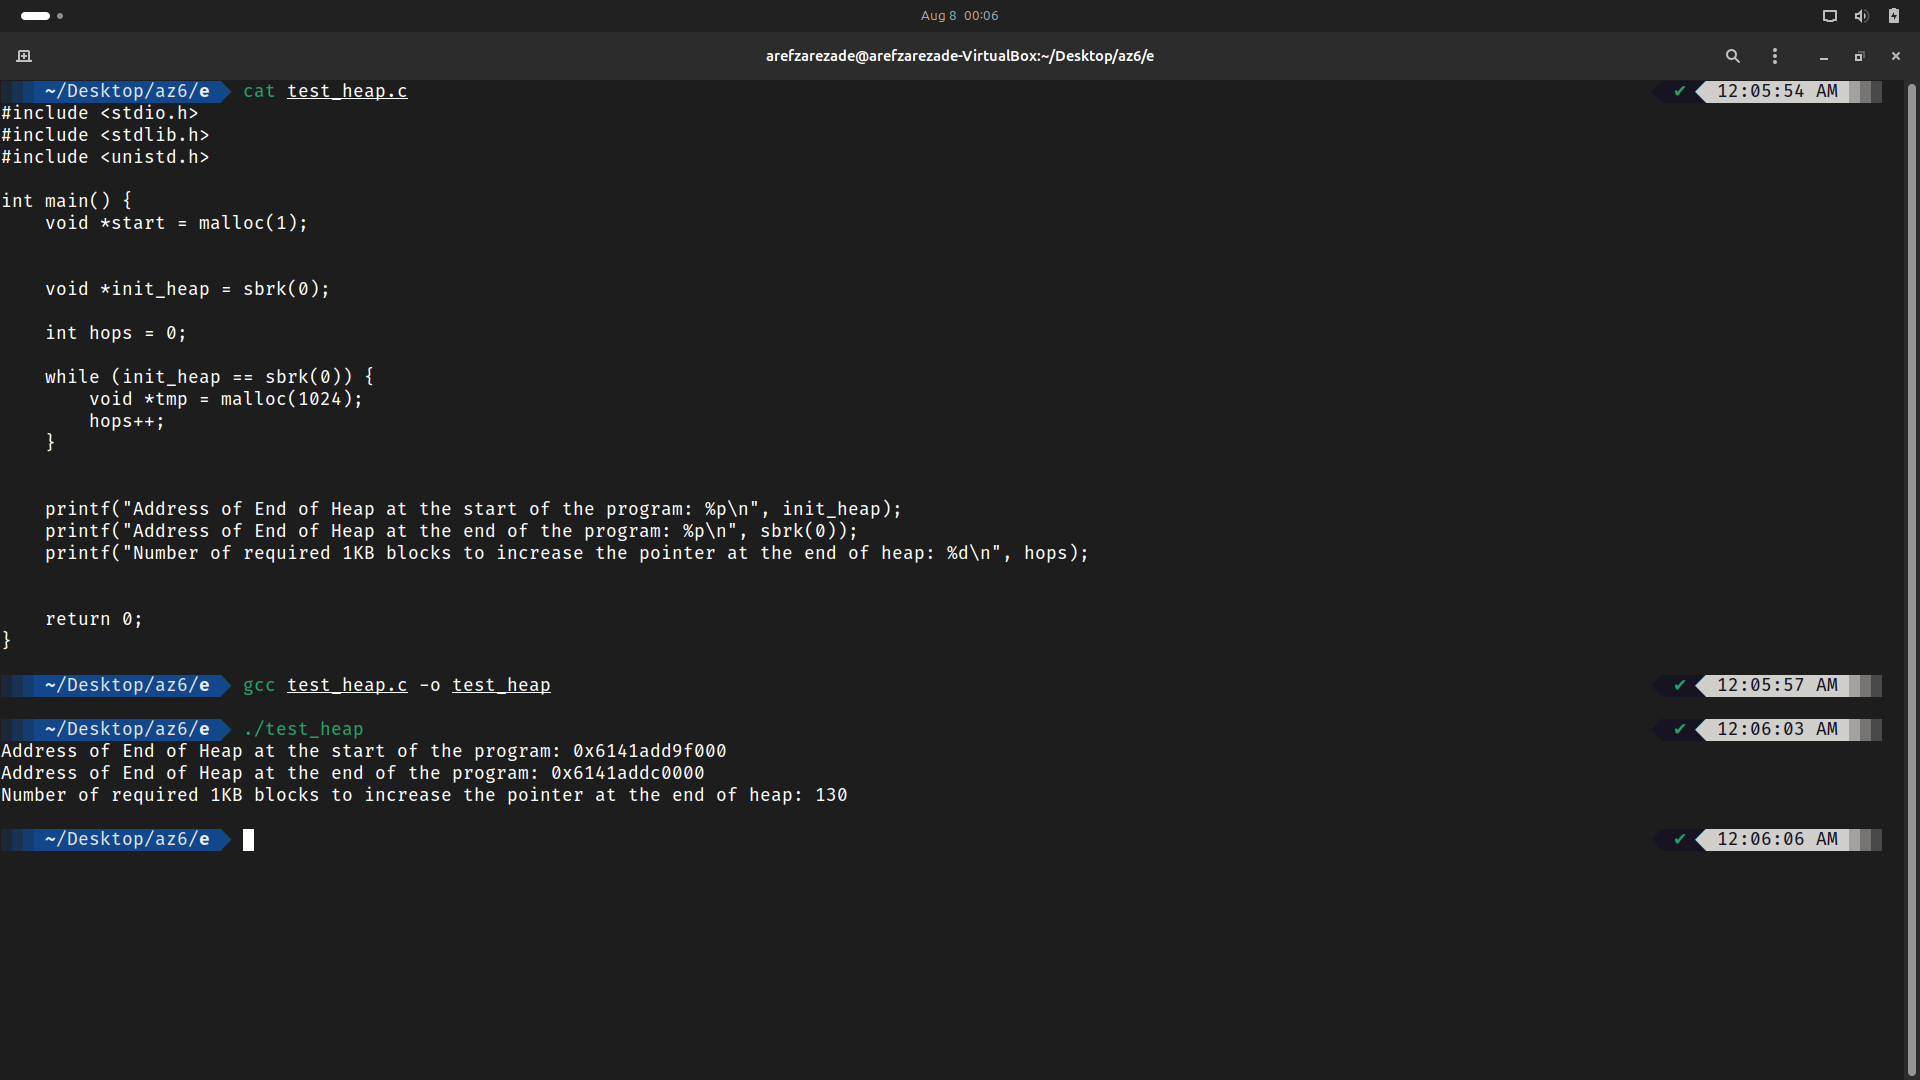
\includegraphics[width=0.8\textwidth]{report6-resources/12.png}
		\caption{تعداد دفعات درخواست \textenglish{1KB} با دستور \textenglish{malloc} برای تغییر آدرس انتهای \textenglish{heap}}
            \label{im12}
	\end{figure}

        همانطور که می‌توان مشاهده کرد، باید چند بار مقدار کوچکی
        (مانند \textenglish{1KB})
        را با دستور
        \textenglish{malloc}
        رزرو کرد تا آدرس انتهای 
        \textenglish{heap}
        تغییر کند. دلیل آن این است که هربار اجرای فراخوانی سیستمی برای رزرو حافظه از لحاظ عملکرد غیر بهینه است، برای همین، دستور 
        \textenglish{malloc}
        در صورت نیاز به حافظه‌ی بیشتر، مقدار نسبتا بزرگی را از سیستم عامل درخواست می‌کند، و با هربار اجرای
        \textenglish{malloc}،
        بخشی از آن حافظه را بر برنامه می‌دهد. اینگونه تعداد دفعات درخواست حافظه از سیستم عامل
        به مراتب کمتر شده و عملکرد برنامه بهتر می‌شود.


        \item 
        برای مشاهده‌ی تغییرات بخش
        \textenglish{stack}، کد موجود در شکل 
        \ref{im13}
        را نوشته‌ایم. این کد، مطابق خواسته‌ی صورت آزمایش، دارای یک تابع بازگشتی است که یک متغیر به نام 
        \textenglish{i}
        ساخته، آدرس آن را چاپ کرده، و سپس دوباره خودش را اجرا می‌کند. همچنین اجرای این تابع را محدود کردیم که بیشتر از تعداد دفعات خواسته شده (که در این مورد 20 بار است) اجرا نشود.

        \begin{figure}[H]
		\centering
		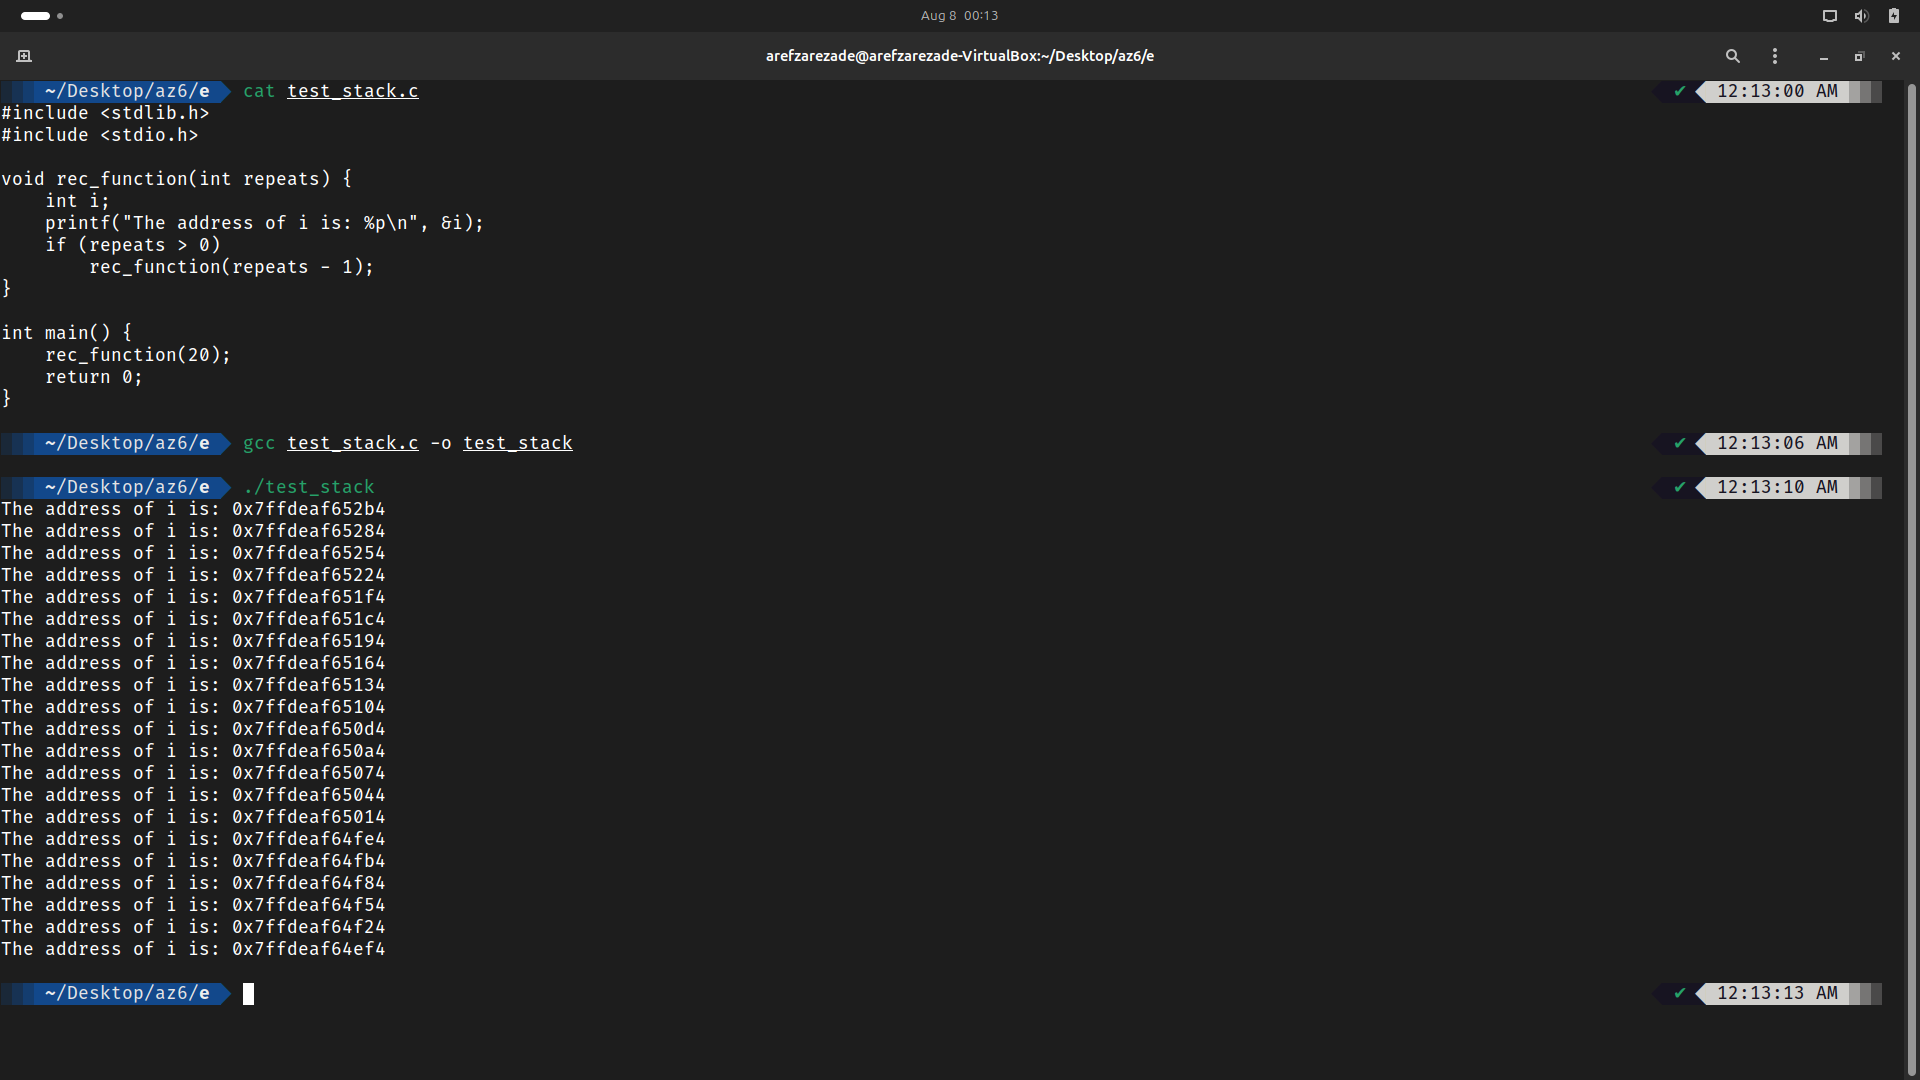
\includegraphics[width=0.8\textwidth]{report6-resources/13.png}
		\caption{مشاهده‌ی رفتار بخش ‌\textenglish{stack} از حافظه}
            \label{im13}
	\end{figure}

        همانطور که از خروجی کد بالا قابل مشاهده است، آدرس متغیر
        \textenglish{i}
        هربار به مقدار ثابتی کاهش می‌یابد. این کاهش بیانگر این است که در هربار اجرای تابع، 
        \textenglish{stack}
        استفاده می‌شود (برای ذخیره‌ی 
        \textenglish{return address}
        و
        \textenglish{stack pointer}
        قبلی و ...). سپس یک مقدار به اندازه‌ی 
        \textenglish{4}
        بایت به متغیر
        \textenglish{i}
        اختصاص داده شده و روند تکرار می‌شود. همچنین اجرای این کد نشان می‌دهد که رشد 
        \textenglish{stack}
        رو به پایین (یا به سمت آدرس‌های کوچکتر) است.
        
        \end{itemize}
    
	
	% ==============================
	% References
	% ==============================
	\newpage
	\begin{LTR}
		\begin{english}
\printbibliography[title={مراجع}]
\end{english}
	\end{LTR}

	
\end{document}

